\subsection{Stato Postazioni}

\begin{figure}[H]
  \centering
    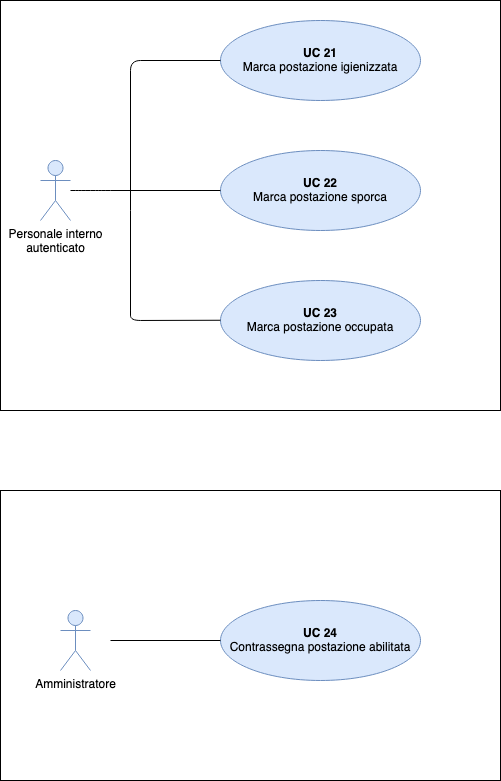
\includegraphics[scale=0.5]{src/CasiDUso/immagini/UC-statoPostazioni.png}
  \caption{UC- Stato prenotazioni}
\end{figure}

Il presente diagramma vuole riassumere la possibilità di prenotazione delle prenotazioni da parte di un utilizzatore dell’applicazione.

\begin{itemize}
\item \textbf{Attori primari:} utente autenticato, igienizzatore, amministratore;
\item \textbf{Descrizione:} l’utente può gestire le postazioni registrate nell’applicazione a cui ha accesso a livello di permessi, aggiungendo, rimuovendo, prenotando ed igienizzando ogni relativa postazione;
\item \textbf{Precondizione:} ogni utente è autenticato, e naviga nell’apposita sezione di gestione delle postazioni;
\item \textbf{Postcondizione:} l’utente ha gestito le proprie postazioni;
\item \textbf{Scenario principale:} 
	\begin{itemize}
		\item l’utente naviga nell’apposita sezione di gestione delle postazioni;
		\item l’utente visualizza e gestisce le postazioni a cui ha accesso.
	\end{itemize}
\end{itemize}


\subsection{UC-20 Marca postazione igienizzata}

\begin{itemize}
\item \textbf{Attori primari:} personale interno autenticato;
\item \textbf{Descrizione:} l'attore può marcare la postazione che sta usando al momento della prenotazione come igienizzata, quindi servibile ed occupabile da un successivo utente;
\item \textbf{Precondizione:} l'attore ha finito di usufruire della postazione; 
\item \textbf{Postcondizione:} l’attore, dall'apposita sezione, marca postazione come igienizzata;
\item \textbf{Scenario principale:} 
	\begin{itemize}
		\item al termine dell'utilizzo della postazione, il sistema invia una domanda di conferma di igienizzazione della postazione;		
		\item l’utente conferma l'avvenuta igienizzazione;
		\item il sistema elabora correttamente la richiesta rendendo disponibile la postazione per una successiva prenotazione.
	\end{itemize}
\end{itemize}

\subsection{UC-21 Marca postazione sporca}

\begin{itemize}
\item \textbf{Attori primari:} personale interno autenticato;
\item \textbf{Descrizione:} al momento della scansione del tag RFID da parte del dispositivo dell'attore, la postazione viene automaticamente marcata come sporca;
\item \textbf{Precondizione:} l'attore ha scansionato il tag RFID; 
\item \textbf{Postcondizione:} il sistema marca la postazione come sporca;
\item \textbf{Scenario principale:} 
		\item il sistema elabora correttamente la richiesta impedendo la prenotazione della postazione da un utente successivo finché non verrà nuovamente igienizzata.
\end{itemize}


\newpage

\subsection{UC-22 Marca postazione occupata}

\begin{itemize}
\item \textbf{Attori primari:} personale interno autenticato;
\item \textbf{Descrizione:} l'attore scansiona con il suo dispositivo il tag RFID, confermando la sua presenza effettiva in postazione;
\item \textbf{Precondizione:} l'attore scansiona il tag RFID;
\item \textbf{Postcondizione:} l'attore ha marcato con successo una postazione come occupata;
\end{itemize}

%\subsubsection{UC-.5 - Conferma prenotazione della postazione}%

%\begin{itemize}%
%\item \textbf{Attori primari:} personale interno autenticato;%
%\item \textbf{Descrizione:} l’utente è tenuto a confermare l’occupazione, e quindi la prenotazione, della postazione in uso;%
%\item \textbf{Precondizione:} l’utente conferma la sua prenotazione dall’apposita schermata pop-up; %
%\item \textbf{Postcondizione:} l’utente ha confermato con successo la prenotazione della postazione;%
%\item \textbf{Scenario principale:} %
%	\begin{itemize}%
%		\item l’utente contrassegna la postazione come occupata;%
%		\item il sistema elabora correttamente la richiesta.%
%	\end{itemize}%
%\end{itemize}%

\subsection{UC-23 Contrassegna postazione abilitata}

\begin{itemize}
\item \textbf{Attori primari:} amministratore;
\item \textbf{Descrizione:} l’amministratore può marcare la postazione precedentemente selezionata come “disabilitata”, nuovamente abilitata, quindi servibile ed occupabile dagli utenti;
\item \textbf{Precondizione:} l’amministratore naviga nell’apposita sezione di gestione della postazione; 
\item \textbf{Postcondizione:} l’amministratore ha marcato con successo una postazione, precedentemente disabilitata, come abilitata;
\item \textbf{Scenario principale:} 
	\begin{itemize}
		\item l’amministratore naviga nell’apposita sezione di gestione della postazione;
		\item l’amministratore contrassegna la postazione come abilitata;
		\item il sistema elabora correttamente la richiesta.
	\end{itemize}
\end{itemize}
